\documentclass[a4paper]{article}
\usepackage{xcolor}        % For gradient colors
\usepackage{graphicx}      % For images
\usepackage{tikz}          % For drawing (without calc)
\usepackage{geometry}      
\geometry{margin=0in}      % Full-page layout

\begin{document}
\pagestyle{empty}  % No page numbers

% === Define Colors ===
\definecolor{DarkBlue}{rgb}{0.1, 0.1, 0.4}
\definecolor{LightBlue}{rgb}{0.6, 0.8, 1.0}
\definecolor{TextOutline}{rgb}{0,0,0}  % Black outline
\definecolor{TextFill}{rgb}{1,1,1}  % White text

\begin{tikzpicture}[remember picture, overlay]

    % --- TOP BLOCK (25% of the page) ---
    \node[anchor=north west, inner sep=0] at (current page.north west) 
        {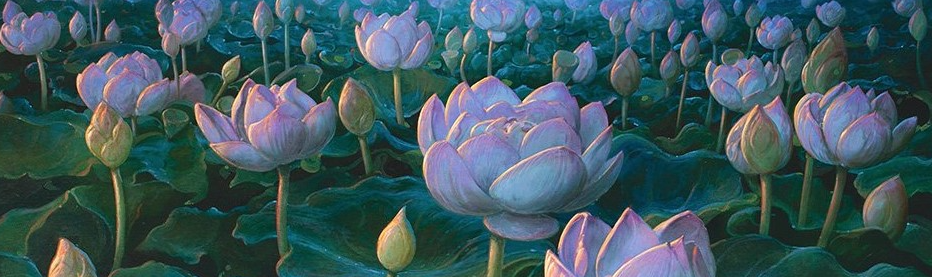
\includegraphics[width=\paperwidth, height=0.25\paperheight]{background.jpg}};

    % --- ROUND CROPPED IMAGE IN THE CENTER ---
    \node[anchor=center] at ([yshift=-0.125\paperheight]current page.north) {
        \begin{tikzpicture}
            \clip (0,0) circle (4cm); % Clip to circular shape
            \node at (0,0) {
\includegraphics[width=8cm]{player.jpg}}; % Keep larger size for cropping effect
        \end{tikzpicture}
    };

    % === NAME AND SURNAME (LEFT SIDE) ===
    \node[anchor=east] at ([xshift=-4.5cm, yshift=-0.125\paperheight]current page.north) {
        \begin{tikzpicture}
            \node[anchor=center, font=\Huge\bfseries, text=TextFill] at (0,0) {Name};
            \node[anchor=center, font=\Huge\bfseries, text=TextFill] at (0,-1) {Surname};
        \end{tikzpicture}
    };

    % === DECK ARCHETYPE (RIGHT SIDE) ===
    \node[anchor=west] at ([xshift=4.5cm, yshift=-0.125\paperheight]current page.north) {
        \begin{tikzpicture}
            \node[anchor=center, font=\Huge\bfseries\itshape, text=TextFill] at (0,0) {Deck};
            \node[anchor=center, font=\Huge\bfseries\itshape, text=TextFill] at (0,-1) {Archetype};
        \end{tikzpicture}
    };

    % --- BOTTOM BLOCK (75% of the page) ---
    \shade[left color=DarkBlue, right color=LightBlue] 
        ([yshift=-0.25\paperheight]current page.north west) 
        rectangle (current page.south east);

    % === MAINBOARD COLUMN (CENTERED AT 25% PAGE WIDTH, AT 27.5% PAGE HEIGHT) ===
    \node[anchor=north] at ([xshift=-0.25\paperwidth, yshift=-0.275\paperheight]current page.north) {
        \begin{tikzpicture}
            \node[anchor=center, font=\Huge\bfseries, text=TextFill] at (0,0) {Mainboard};
            % Placeholder List
            \node[anchor=north, font=\Large\bfseries, text=TextFill] at (0,-1) {
                \begin{tabular}{c}
                    Card 1 \\
                    Card 2 \\
                    Card 3 \\
                    Card 4 \\
                    Card 5 \\
                    Card 6 \\
                    Card 7 \\
                    Card 8 
                \end{tabular}
            };
        \end{tikzpicture}
    };

    % === SIDEBOARD COLUMN (CENTERED AT 75% PAGE WIDTH, AT 27.5% PAGE HEIGHT) ===
    \node[anchor=north] at ([xshift=0.25\paperwidth, yshift=-0.275\paperheight]current page.north) {
        \begin{tikzpicture}
            \node[anchor=center, font=\Huge\bfseries, text=TextFill] at (0,0) {Sideboard};
            % Placeholder List
            \node[anchor=north, font=\Large\bfseries, text=TextFill] at (0,-1) {
                \begin{tabular}{c}
                    Card A \\
                    Card B \\
                    Card C \\
                    Card D \\
                    Card E \\
                    Card F \\
                    Card G \\
                    Card H 
                \end{tabular}
            };
        \end{tikzpicture}
    };

\end{tikzpicture}

\end{document}
